%%%%%%%%%%%%%%%%%%%%%%%%%%%%%%%%%%%%%%%%
% datoteka diploma.tex
%
% vzorčna datoteka za pisanje diplomskega dela v formatu LaTeX
% na UL Fakulteti za računalništvo in informatiko
%
% vkup spravil Gašper Fijavž, december 2010
% 
%
%
% verzija 12. februar 2014 (besedilo teme, seznam kratic, popravki Gašper Fijavž)
% verzija 10. marec 2014 (redakcijski popravki Zoran Bosnić)
% verzija 11. marec 2014 (redakcijski popravki Gašper Fijavž)
% verzija 15. april 2014 (pdf/a 1b compliance, not really - just claiming, Damjan Cvetan, Gašper Fijavž)
% verzija 23. april 2014 (privzeto cc licenca)
% verzija 16. september 2014 (odmiki strain od roba)
% verzija 28. oktober 2014 (odstranil vpisno številko)
% verija 5. februar 2015 (Literatura v kazalu, online literatura)
% verzija 25. september 2015 (angl. naslov v izjavi o avtorstvu)
% verzija 26. februar 2016 (UL izjava o avtorstvu)
% verzija 16. april 2016 (odstranjena izjava o avtorstvu)
% verzija 5. junij 2016 (Franc Solina dodal vrstice, ki jih je označil s svojim imenom)
% verzija junij 2018 (Polona Oblak, I?RM predloga)
\documentclass[a4paper, 12pt]{book}
%\documentclass[a4paper, 12pt, draft]{book}  Nalogo preverite tudi z opcijo draft, ki vam bo pokazala, katere vrstice so predolge!
\usepackage[utf8x]{inputenc}   % omogoča uporabo slovenskih črk kodiranih v formatu UTF-8
\usepackage[slovene,english]{babel}    % naloži, med drugim, slovenske delilne vzorce
\usepackage[pdftex]{graphicx}  % omogoča vlaganje slik različnih formatov
\usepackage{fancyhdr}          % poskrbi, na primer, za glave strani
\usepackage{amssymb}           % dodatni simboli
\usepackage{amsmath}           % eqref, npr.
%\usepackage{hyperxmp}
\usepackage[hyphens]{url}  % dodal Solina
\usepackage{comment}       % dodal Solina
\usepackage[pdftex, colorlinks=true,
						citecolor=black, filecolor=black, 
						linkcolor=black, urlcolor=black,
						pagebackref=false, 
						pdfproducer={LaTeX}, pdfcreator={LaTeX}, hidelinks]{hyperref}
\usepackage{color}       % dodal Solina
\usepackage{soul}       % dodal Solina
%%%%%%%%%%%%%%%%%%%%%%%%%%%%%%%%%%%%%%%%
%	DIPLOMA INFO
%%%%%%%%%%%%%%%%%%%%%%%%%%%%%%%%%%%%%%%%
\newcommand{\ttitle}{Povezovanje klastrov Kubernetes}
\newcommand{\ttitleEn}{Connecting Kubernetes clusters}
\newcommand{\tsubject}{\ttitle}
\newcommand{\tsubjectEn}{\ttitleEn}
\newcommand{\tauthor}{Jakob Hostnik}
\newcommand{\tkeywords}{gruča, oblak, Kubernetes, računalniški klaster, povezovanje klastrov, mreža klastrov,  KubeFed, Cilium, GitOps, ArgoCD}
\newcommand{\tkeywordsEn}{cluster, cloud, Kubernetes, computer cluster, connecting clusters, cluster mesh,  KubeFed, Cilium, GitOps, ArgoCD}
%%%%%%%%%%%%%%%%%%%%%%%%%%%%%%%%%%%%%%%%
%	HYPERREF SETUP
%%%%%%%%%%%%%%%%%%%%%%%%%%%%%%%%%%%%%%%%
\hypersetup{pdftitle={\ttitle}}
\hypersetup{pdfsubject=\ttitleEn}
\hypersetup{pdfauthor={\tauthor, jakob@hostnik.si}}
\hypersetup{pdfkeywords=\tkeywordsEn}
%%%%%%%%%%%%%%%%%%%%%%%%%%%%%%%%%%%%%%%%
% postavitev strani
%%%%%%%%%%%%%%%%%%%%%%%%%%%%%%%%%%%%%%%%  
\addtolength{\marginparwidth}{-20pt} % robovi za tisk
\addtolength{\oddsidemargin}{40pt}
\addtolength{\evensidemargin}{-40pt}
\renewcommand{\baselinestretch}{1.3} % ustrezen razmik med vrsticami
\setlength{\headheight}{15pt}        % potreben prostor na vrhu
\renewcommand{\chaptermark}[1]%
{\markboth{\MakeUppercase{\thechapter.\ #1}}{}} \renewcommand{\sectionmark}[1]%
{\markright{\MakeUppercase{\thesection.\ #1}}} \renewcommand{\headrulewidth}{0.5pt} \renewcommand{\footrulewidth}{0pt}
\fancyhf{}
\fancyhead[LE,RO]{\sl \thepage} 
%\fancyhead[LO]{\sl \rightmark} \fancyhead[RE]{\sl \leftmark}
\fancyhead[RE]{\sc \tauthor}              % dodal Solina
\fancyhead[LO]{\sc Diplomska naloga}     % dodal Solina
\newcommand{\BibTeX}{{\sc Bib}\TeX}
%%%%%%%%%%%%%%%%%%%%%%%%%%%%%%%%%%%%%%%%
% naslovi
%%%%%%%%%%%%%%%%%%%%%%%%%%%%%%%%%%%%%%%%  
\newcommand{\autfont}{\Large}
\newcommand{\titfont}{\LARGE\bf}
\newcommand{\clearemptydoublepage}{\newpage{\pagestyle{empty}\cleardoublepage}}
\setcounter{tocdepth}{1}	      % globina kazala
%%%%%%%%%%%%%%%%%%%%%%%%%%%%%%%%%%%%%%%%
% konstrukti
%%%%%%%%%%%%%%%%%%%%%%%%%%%%%%%%%%%%%%%%  
\newtheorem{izrek}{Izrek}[chapter]
\newtheorem{trditev}{Trditev}[izrek]
\newenvironment{dokaz}{\emph{Dokaz.}\ }{\hspace{\fill}{$\Box$}}
%%%%%%%%%%%%%%%%%%%%%%%%%%%%%%%%%%%%%%%%%%%%%%%%%%%%%%%%%%%%%%%%%%%%%%%%%%%%%%%
%% PDF-A
%%%%%%%%%%%%%%%%%%%%%%%%%%%%%%%%%%%%%%%%%%%%%%%%%%%%%%%%%%%%%%%%%%%%%%%%%%%%%%%
%%%%%%%%%%%%%%%%%%%%%%%%%%%%%%%%%%%%%%%% 
% define medatata
%%%%%%%%%%%%%%%%%%%%%%%%%%%%%%%%%%%%%%%% 
\def\Title{\ttitle}
\def\Author{\tauthor, jakob@hostnik.si}
\def\Subject{\ttitleEn}
\def\Keywords{\tkeywordsEn}
%%%%%%%%%%%%%%%%%%%%%%%%%%%%%%%%%%%%%%%% 
% \convertDate converts D:20080419103507+02'00' to 2008-04-19T10:35:07+02:00
%%%%%%%%%%%%%%%%%%%%%%%%%%%%%%%%%%%%%%%% 
\def\convertDate{%
    \getYear
}
{\catcode`\D=12
 \gdef\getYear D:#1#2#3#4{\edef\xYear{#1#2#3#4}\getMonth}
}
\def\getMonth#1#2{\edef\xMonth{#1#2}\getDay}
\def\getDay#1#2{\edef\xDay{#1#2}\getHour}
\def\getHour#1#2{\edef\xHour{#1#2}\getMin}
\def\getMin#1#2{\edef\xMin{#1#2}\getSec}
\def\getSec#1#2{\edef\xSec{#1#2}\getTZh}
\def\getTZh +#1#2{\edef\xTZh{#1#2}\getTZm}
\def\getTZm '#1#2'{%
    \edef\xTZm{#1#2}%
    \edef\convDate{\xYear-\xMonth-\xDay T\xHour:\xMin:\xSec+\xTZh:\xTZm}%
}
\expandafter\convertDate\pdfcreationdate 
%%%%%%%%%%%%%%%%%%%%%%%%%%%%%%%%%%%%%%%%
% get pdftex version string
%%%%%%%%%%%%%%%%%%%%%%%%%%%%%%%%%%%%%%%% 
\newcount\countA
\countA=\pdftexversion
\advance \countA by -100
\def\pdftexVersionStr{pdfTeX-1.\the\countA.\pdftexrevision}
%%%%%%%%%%%%%%%%%%%%%%%%%%%%%%%%%%%%%%%%
% XMP data
%%%%%%%%%%%%%%%%%%%%%%%%%%%%%%%%%%%%%%%%  
\usepackage{xmpincl}
\includexmp{pdfa-1b}
%%%%%%%%%%%%%%%%%%%%%%%%%%%%%%%%%%%%%%%%
% pdfInfo
%%%%%%%%%%%%%%%%%%%%%%%%%%%%%%%%%%%%%%%%  
\pdfinfo{%
    /Title    (\ttitle)
    /Author   (\tauthor, jakob@hostnik.si)
    /Subject  (\ttitleEn)
    /Keywords (\tkeywordsEn)
    /ModDate  (\pdfcreationdate)
    /Trapped  /False
}
%%%%%%%%%%%%%%%%%%%%%%%%%%%%%%%%%%%%%%%%%%%%%%%%%%%%%%%%%%%%%%%%%%%%%%%%%%%%%%%
%%%%%%%%%%%%%%%%%%%%%%%%%%%%%%%%%%%%%%%%%%%%%%%%%%%%%%%%%%%%%%%%%%%%%%%%%%%%%%%
\begin{document}
\selectlanguage{slovene}
\frontmatter
\setcounter{page}{1} %
\renewcommand{\thepage}{}       % preprecimo težave s številkami strani v kazalu
\newcommand{\sn}[1]{"`#1"'}                    % dodal Solina (slovenski narekovaji)
%%%%%%%%%%%%%%%%%%%%%%%%%%%%%%%%%%%%%%%%
%naslovnica
 \thispagestyle{empty}%
   \begin{center}
    {\large\sc Univerza v Ljubljani\\%
      Fakulteta za računalništvo in informatiko\\%
      Fakulteta za matematiko in fiziko}%
    \vskip 10em%
    {\autfont \tauthor\par}%
    {\titfont \ttitle \par}%
    {\vskip 3em \textsc{DIPLOMSKO DELO\\[5mm]        
    INTERDISCIPLINARNI UNIVERZITETNI\\ ŠTUDIJSKI PROGRAM PRVE STOPNJE\\ RAČUNALNIŠTVO IN MATEMATIKA}\par}%
    \vfill\null%
    {\large \textsc{Mentor}: izr. prof. dr. Mojca Ciglarič \par}%
   {\large \textsc{Somentor}:  asist. dr. Matjaž Pančur \par}%
    {\vskip 2em \large Ljubljana, 2021 \par}%
\end{center}
% prazna stran
%\clearemptydoublepage      % dodal Solina (izjava o licencah itd. se izpiše na hrbtni strani naslovnice)
%%%%%%%%%%%%%%%%%%%%%%%%%%%%%%%%%%%%%%%%
%copyright stran
\thispagestyle{empty}
\vspace*{8cm}
\noindent
{\sc Copyright}. 
Rezultati diplomske naloge so intelektualna lastnina avtorja in Fakultete za računalništvo in informatiko Univerze v Ljubljani.
Za objavo in koriščenje rezultatov diplomske naloge je potrebno pisno privoljenje avtorja, Fakultete za računalništvo in informatiko ter mentorja.
\begin{center}
\mbox{}\vfill
\emph{Besedilo je oblikovano z urejevalnikom besedil \LaTeX.}
\end{center}
% prazna stran
\clearemptydoublepage
%%%%%%%%%%%%%%%%%%%%%%%%%%%%%%%%%%%%%%%%
% stran 3 med uvodnimi listi
\thispagestyle{empty}
\vspace*{4cm}
\noindent
Fakulteta za računalništvo in informatiko izdaja naslednjo nalogo:
\medskip
\begin{tabbing}
\hspace{32mm}\= \hspace{6cm} \= \kill
Tematika naloge:
\end{tabbing}
TODO
Besedilo teme diplomskega dela študent prepiše iz študijskega informacijskega sistema, kamor ga je vnesel mentor. V nekaj stavkih bo opisal, kaj pričakuje od kandidatovega diplomskega dela. Kaj so cilji, kakšne metode uporabiti, morda bo zapisal tudi ključno literaturo.
\vspace{15mm}
\vspace{2cm}
% prazna stran
\clearemptydoublepage
% zahvala
\thispagestyle{empty}\mbox{}\vfill\null\it%
\noindent
Na tem mestu bi se zahvalil mentorici izr. prof. dr. Mojca Ciglarič za pripravljenost in mentorstvo.
Zahvalil bi se tudi somentorju asist. dr. Matjažu Pančurju za vse nasvete in pomoč pri pisanju diplomske naloge.
Zahvala pa gre tudi moji ženi, staršem, bratom, sestram in prijateljem za podporo in spodbudo pri študiju.
\rm\normalfont
% prazna stran
\clearemptydoublepage
%%%%%%%%%%%%%%%%%%%%%%%%%%%%%%%%%%%%%%%%
% posvetilo, če sama zahvala ne zadošča :-)
\thispagestyle{empty}\mbox{}{\vskip0.20\textheight}\mbox{}\hfill\begin{minipage}{0.55\textwidth}%
Mami Lučki.
\normalfont\end{minipage}
% prazna stran
\clearemptydoublepage
%%%%%%%%%%%%%%%%%%%%%%%%%%%%%%%%%%%%%%%%
% kazalo
\pagestyle{empty}
\def\thepage{}% preprecimo tezave s stevilkami strani v kazalu
\tableofcontents{}
% prazna stran
\clearemptydoublepage
%%%%%%%%%%%%%%%%%%%%%%%%%%%%%%%%%%%%%%%%
% seznam kratic
\chapter*{Seznam uporabljenih kratic}  % spremenil Solina, da predolge vrstice ne gredo preko desnega roba
\noindent\begin{tabular}{p{0.1\textwidth}|p{.4\textwidth}|p{.4\textwidth}}    % po potrebi razširi prvo kolono tabele na račun drugih dveh!
  {\bf kratica} & {\bf angleško}                             & {\bf slovensko} \\ \hline
  {\bf CRD} & custom resource definition & definicija tipov po meri \\
  {\bf DNS} & domain name system & sistem za upravljanje domen \\
  {\bf IP} & internet protocol & internetni protokol \\
  {\bf HA} & high availability & visoka dosegljivost \\
  {\bf GA} & general availability & splošna dostopnost \\
  {\bf VPN} & virtual private network & virtualno privatno omrežje \\
\end{tabular}
% prazna stran
\clearemptydoublepage
%%%%%%%%%%%%%%%%%%%%%%%%%%%%%%%%%%%%%%%%
% povzetek
\addcontentsline{toc}{chapter}{Povzetek}
\chapter*{Povzetek}
\noindent\textbf{Naslov:} \ttitle
\bigskip

\noindent\textbf{Avtor:} \tauthor
\bigskip
%\noindent\textbf{Povzetek:} 
\noindent 

Več računalnikov povezujemo v skupine predvsem zaradi zagotavljanja večje zmogljivosti in stabilnosti.
V zadnjih letih je bil na tem področju narejen zelo velik napredek in razvoj.
Tako je nastal tudi sistem Kubernetes, ki je zaradi svoje popularnosti postal svetovni standard za upravljanje klastrov, orkestracijo kontejnerjev.
A zelo pogosto en sam računalniški klaster ni dovolj.
To se zgodi v primerih, ko imamo težave z dragim prenosom podatkov, preveliko latenco, do naših uporabnikov,  želimo še bolj povečati stabilnost ali varnost našega sistema.
Primerov uporabe je veliko in v diplomski nalogi si bomo pogledali nekaj najpogostejših.
Pogledali si bomo, ozadje povezovanja klastrov postavljenih s sistemom Kubernetes in kakšne pristope lahko uporabimo.
Lotili se bomo implementacije in reševanja problemov skozi nekaj pogostih problemov v resničnem svetu.
Poseben poudarek pa bomo dali tudi sinhronizaciji podatkov, saj je to eden težjih delov pri upravljanju večih računalniških klastrov.
Ugotovimo, da nam lahko sodobne metode povezovanja klastrov zelo olajšajo njihovo upravljanje in preprosto rešijo tudi težje probleme sinhronizacije podatkov.

\bigskip
\noindent\textbf{Ključne besede:} \tkeywords.
% prazna stran
\clearemptydoublepage
%%%%%%%%%%%%%%%%%%%%%%%%%%%%%%%%%%%%%%%%
% abstract
\selectlanguage{english}
\addcontentsline{toc}{chapter}{Abstract}
\chapter*{Abstract}
\noindent\textbf{Title:} \ttitleEn
\bigskip
\noindent\textbf{Author:} \tauthor
\bigskip
%\noindent\textbf{Abstract:} 
\noindent 

TODO
This sample document presents an approach to typesetting your BSc thesis using \LaTeX. 
A proper abstract should contain around 100 words which makes this one way too short.

\bigskip
\noindent\textbf{Keywords:} \tkeywordsEn.
\selectlanguage{slovene}
% prazna stran
\clearemptydoublepage
%%%%%%%%%%%%%%%%%%%%%%%%%%%%%%%%%%%%%%%%
\mainmatter
\setcounter{page}{1}
\pagestyle{fancy}
\chapter{Uvod}
\label{uvod}
\section{Motivacija}
Glede orkestracije kontainerjev je bil v zadnjih nekaj letih narejen zelo velik preboj. 
V postopku tega preboja se je razvil tudi Kubernetes API, ki je na tem področu rešil marsikatero težavo.
Kubernetes  je univerzalni način, ki nam omogoča, da več račualnikov povežemo v klaster, ki deluje kot ena samostojna enota. 
To reši marsikatero težavo v računalništvu in vsaj teoretično je to dovolj, da imamo visoko dosegljivost (HA) naših storitev ~\cite{mastering-Kubernetes} in sinhrono delovanje večih računalnikov.
A industrija je zelo hitro ugotovila, da obstaja kar nekaj primerov, ko ni dovolj, da ena skupina računalnikov deluje kot celota ampak bi želeli med seboj povezujemo tudi te skupine.
Ta problem se je do sedaj reševalo na več različnih načinov.
Je pa v zadnjem času tudi Kubernetes začel bolj aktivno problem reševati celostno.
Začel je s propadlim projektom Federation 1, zdaj pa se zdi, kot da bo Federation 2 ali KubeFed uspešno prešel iz alfa verzije v beta.
Skratka v računalništvi je na tem področju zelo veliko zanimanja in razvoja.
\section{Cilj in vsebina naloge}
V tem diplomskem delu si bomo pogledali nekaj o reševanju tega problema, Kubernetesu in reševanju resničnih problemov v industriji. 
Za vsakega od primerov si bomo pogledali kako se ta problem rešuje v Kubernetes okolju z uporabo orodja KubeFed in kako bi sinhronizirali tudi podatke.
\subsection{Prevelika latenca}
Ko spletne aplikacije postanejo bolj globalne zelo hitro opazimo, da uporabniki, ki so na drugi celini kot naši strežniki preživijo veliko več časa pred ikonami za nalaganje, saj podatki do njih potujejo dalj časa.
Ta problem je rešljiv na način, da postavimo še en klaster bližje naših uporanbikov.
Naprimer en klaster na celino.
Tu pa zelo pogosto želimo, da se podatki sinhronizirajo.
Zavedati se moramo, da strežniki v klastru zelo veliko komunicirajo zato morajo biti tudi fizično blizu skupaj. 
To je tudi ena glavnih omejitev, da ne moremo vseh klastrov povezati v en večji klaster.
\begin{figure}[h]
\begin{center}
  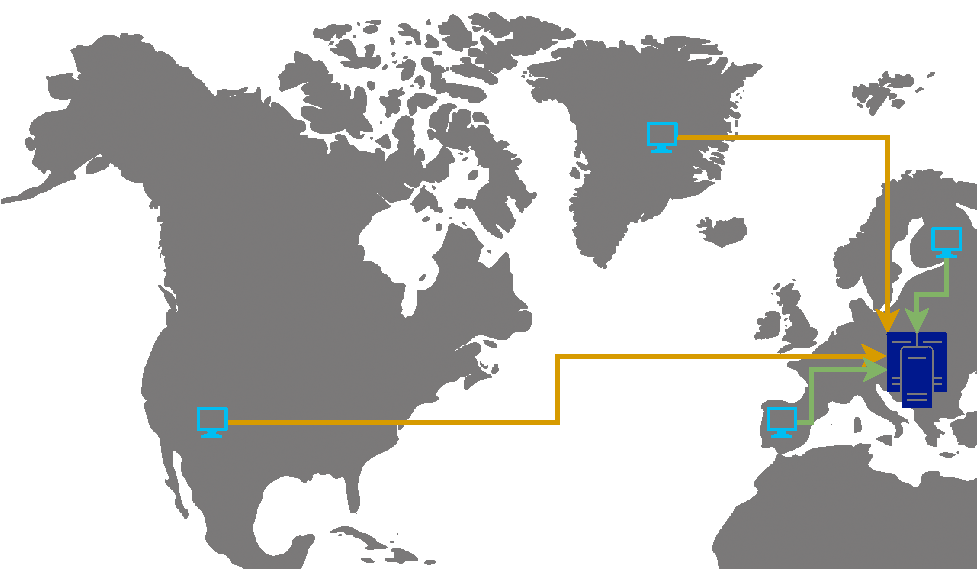
\includegraphics[width=1.0\textwidth]{images/problem-prevelike-latence.pdf}
\end{center}
\caption{Problem prevelike latence.}
\label{problem-prevelike-latence}
\end{figure}
\subsection{Viša dosegljivost}
Vsakih nekaj let se zgodi da slišimo novico ko iz interneta izpade kakšen podatkovni center. 
To se lahko zgodi iz več razlogov, najpogostejša pa sta naravne nesreče in napake na sistemu.
Če gre v takšnem primeru za večjega oblačnega ponudnika se to pozna tako, da je nezanemarljiv del interneta nedosegljiv.
Izpadi posameznih klastrov pa se toliko pogosteje dogajajo, če gre za manjše ponudnike ali pa so naši strežniki v bolj nestabilnih okoljih. 
V splošnem se problem reši tako, da se namesti v vsak podatkovni center, skupino strežnikov en klaster.
\subsection{Izolacija aplikacije}
Ko govorimo o izolaciji aplikacije se ponavadi nanašamo na varnost pri vdoru, ali pa na večjo dosegljivost.
Glede izolacije spletnih aplikacij smo z uporabo Kubernetesa naredili že kar nekaj korakov.
Naprimer vsaka aplikacija lahko teče v svojem kontejnerju, tudi v imenskem prostoru.
Lahko jo celo izoliramo samo na določera vozlišča.
A vseeno se v Kubernetesu dogajajo problemi, ki naredijo cel klaster nedosegljiv.
Kaj takšnega se najpogosteje zgodi med posodabljanjem celega klastra.
Z varnostnega vidika pa ponavadi mislimo na dejstvo, da če nekomu uspe serija napadov in se uspešno polasti enega samega vozlišča si začne lastiti cel klaster.
Torej ima dostop tudi do vseh drugih aplikacij.
Če imamo vsako od naših aplikacij v svojem klastru pa se temu izognemo.
\subsection{Drag prenos podatkov}
Če se spustimo iz jedra računalniškega oblaka na njegov rob pa tam srečamo cel kup zanimivih problemov. 
Na robu oblaka smo takrat, ko govorimo o delu naše aplikaije, ki se izvaja stran od centralnih aplikacij, ki so vedno doseljive.
Takšen primer so naprimer mikro podatkovni centri in klastri, na majhnih računalnikih kot naprimer raspberry pi.
Če naša aplikacija uporablja takšne klastre je potrbno tudi njihovo sinhrono delovanje.
Takšni majhni klastri so poleg ze znanega problema prevelike razdalje ponavadi obsojeni, da s centralinimi strežniki komunicirajo samo minimalno, saj zelo pogosto za prenost podatkov uporabljajo draga mobilna omrežja.
\subsection{Razdeljevanje dela po različnih lokacijah}
Na robu oblaka pa se ponaavdi srečamo ne samo z omejenim komuniiranjem s centralnim strežnikom ampak tudi zmanjšano dosegljivostjo in tudi zmogljivostjo naprav.
Torej če ima en klaster manj dela kot drugi lahko delež tega prenese na druge klastre.
\chapter{Problem povezovanje klastrov}
Računalniški klaster je skupina računalnikov, ki zaradi večje zanesljivosti in zmogljivosti skupaj opravlja določene storitve.
Zaradi praktičnosti, pa so te storitve ponavadi napisane tako, da vsako storitev sestavlja več programov, ki tečejo v kontejnerjih.

Problem povezovanja večih računalniških klastrov je v svetu prisoten že kar nekaj časa.
Ko postavimo klaster, želimo da več računalnikov deluje kot eno, a z veliko večjo zanesljivostjo, stabilnostjo in zmogljivostjo.
Obstajajo primeri, ko bi radi med seboj povezali računalnike, a jih zaradi razdalje ali druačnih ovir ne moremo povezati v en tesno povezan klaster.
V takšnih primerih ponavadi lahko računalnike povežemo v več tesno povezanih klastrov, te pa potem na različne načine povežemo šibkeje.

Ko govorimo o tesni povezanosti znotraj klastra ponavadi pričakujemo, da vsako vozlišče vidi vsako drugo, da vsak kontejner lahko komunicira z vsakim kontejnerjem, da so vozlišča v istem omrežju, da je povezava med vozlišči hitra, poceni in zanesljiva. 
Pričakujemo, da sistem, ki ga uporabljamo za klaster omogoča, razporejanje zaželenih storitev in kontejnerjev med vozlišči in v primeru izpada vozlišča to vozlišča odstrani iz sistema in storitve s tega vozlišča prerazporedi na preostala vozlišča.

Ko pa govorimo o šibki povezanosti med različnimi klastri pa zaradi omejitev redko pričakujemo komunikacijo vsakega vozlišča z vsakim.
Zelo pogosto je povezava med vozlišči počasna, nezanesljiva in draga.
Ponavadi je vsak klaster v svojem omrežju in je nedosegljiv ostalim klastrom.
Pričakujemo, da vsak klaster skrbi za svoja vozlišča in da ohranja svoje storitve in kntejnerje v delovanju.
Od sistema za povezovanje klastrov pa si želimo, da nam omogoča centralni nadzor nad storitvami v klastrih, prerazporejanje teh storitev med klastri, dinamično odkrivanje drugih klastrov in njihovih storitev, izločanje nedosegljivih klastrov, povezljivost med vsemi vozlišči in kontejnerji, četudi so vozlišča v različnih omrežjih.

\begin{figure}[h]
\begin{center}
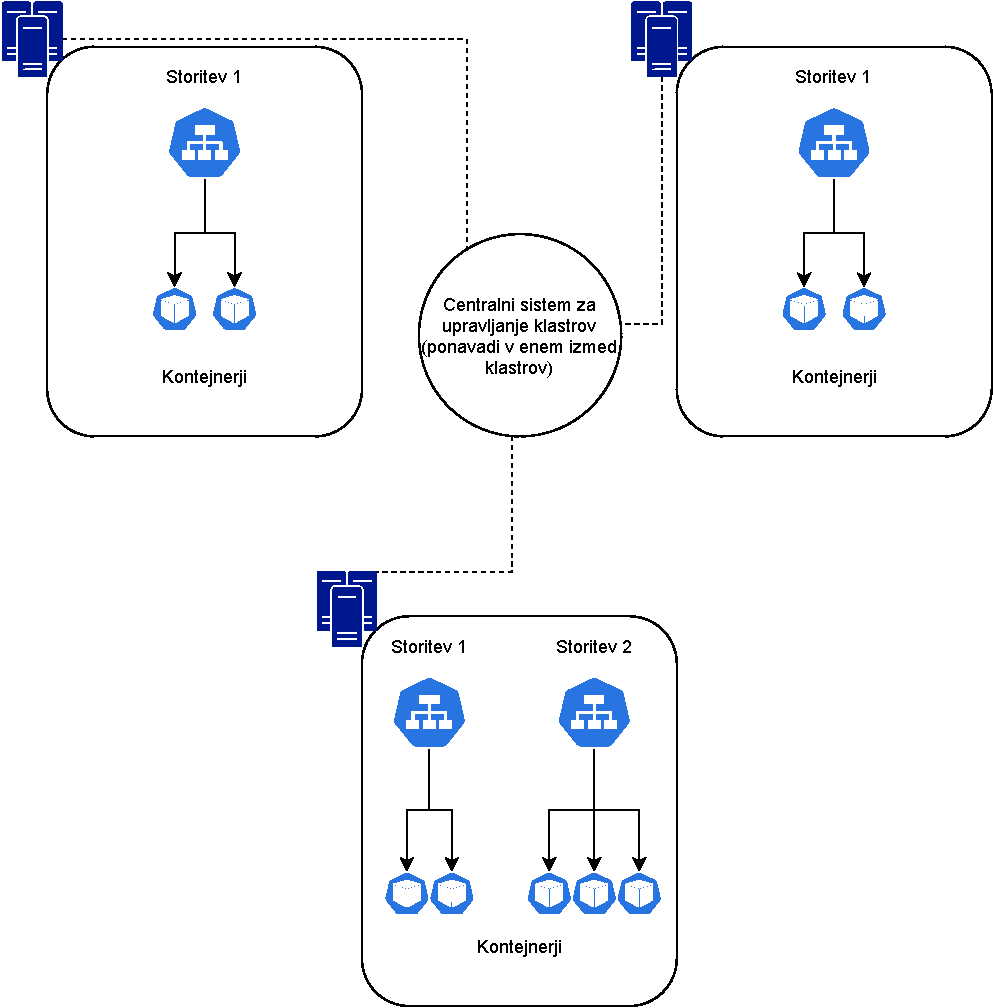
\includegraphics[width=1.0\textwidth]{images/primer-povezanih-klastrov.pdf}
\end{center}
\caption{Primer povezanih večih klastrov.}
\label{problem-povezanih-klastrov}
\end{figure}

\chapter{Kubernetes}
\label{Kubernetes}
Kubernetes je REST API in trenutno obstaja že več kot 72 implementacij tega API-ja. Ko se bomo sklicevali na Kubernetes v tem dokumentu bomo imeli v mislih implementacijo Kubernetesa.
\section{Zgodovina}
Leta 2014 je Google objavil in odprl kodo od projekta Kubernetes~\cite{what-is-Kubernetes}.
Gre za program bil ustvarjen z namenom, da poenostavi upravljanje kontejnerjev in večjih računalniških klastrov v produkcijskih okoljih.
A to vseeno niso pravi začetki Kubernetesa.
Začelo se je leta 2003, ko je Google začel z razvojem sistema za upravljanje njihovih internih klastrov Borg.
Kasneje leta 2013 je google predstavil sistem Omega.
Leta 2014 pa je google objavil projekt Kubernetes, kot odprtokodno verzijo borga.
Kasneje je upravljanje prevzela organizacija Cloud Native Computing Fundation.
\section{Osnoovni pojmi}
Kubernetes API nam omogoča, da v Kubernetes shranjujemo najrazličnejše objekte.
Takšne, ki so v naprej definirani ali pa smo jih definirali sami (CRD).
Najpogostejši v naprej definirani objekti, ki se pojavijo v Kubernetesu so pod, service, deployment, statefulset in objekti za delo z diski.
\begin{figure}[h]
\begin{center}
\includegraphics[width=1.0\textwidth]{images/Kubernetes-simple-schema.pdf}
\end{center}
\caption{Primer delovanja Kubernetes objektov.}
\label{problem-povezanih-klastrov}
\end{figure}
\subsection{Pod~\cite{pod}}
Objekt pod ponavadi predstavlja neko instanco mikrostoritve.
Gre za najmanjšo enoto v Kubernetesu, ki lahko teče v klastru.
Je sestavljen iz enega ali več kontejnerjev ki si delijo diske in omrežni vmesnik.
To pomeni, da imajo skupen IP in se obnašajo podobno kot izolirani procesi na istem računalniku.
\subsection{Service~\cite{service}}
Objekt service ponavadi označuje vse pode ene mikrostoritve.
Kubernetes iz objekta v internem DNS ustvari domeno za mikrostoritev in dinamično razvršča promet med našimi podi.
service uporabljamo tako, da namesto pošiljanja zahtevkov direktno na IP naslov Poda, delamo klice na ustvarjeno domeno.
Takšen zahtevek potem dobi en izmed označenih podov v objektu service.
\subsection{Deployment~\cite{deployment}}
deployment je objekt, ki mu podamo število željenih objektov pod in predlogo za njihovo izdelavo.
Potem pa interne storitve Kubernetesa zagotavljajo, da bo obstajalo toliko takšnih objektov tipa pod kot smo navedli v deploymentu.
Takšno stanje se poizkuša ohranjati tudi ob raznih težavah in izpadih vozlišč.
\subsection{StatefulSet~\cite{statefulset}}
Objekt zelo podoben deploymentu, le da statefulset vsaki replikaciji poda dodeli unikatno številno. 
pod, ki se ustvari s to številko ohranja diske in IP naslov in domeno.
Pomembna razlika med objektoma deployment in statefulset pa je tudi v polju volumeClaimTemplate.
statefulset omogoča vsakemu podu, da si ustvari in uporablja svoj disk.
statefulset se najpogosteje uporablja za podatkovne baze in podobne storitve, ki morajo ohranjati stanja.
\chapter{Povezovanje klastrov Kubernetes }
Ko postavimo več različnih klastrov imamo vedno možnost, da upravljamo vsakega posebej~\cite{difference-multi-cluster}.
A takšen pristop zelo kmalu odpove, če imamo takšnih klastrov res veliko.
Ko govorimo o sistemu, ki ga uporabljamo za upravljanje večih klastrov, najpogosteje pričakujemo možnost prenašanje objektov med klastri.
Tako lahko objekt definiramo samo enkrat in bo naš sistem ta objekt ustvaril v klastrih, kjer to želimo.
Odvisno od naših potreb pa si lahko želimo tudi, da nam sistem omogoča dinamično odkrivanje servicov z enako definicijo v različnih klastrih, komunikacijo med servici v različnih klastrih, dinamično odkrivanje podov med klastri in komunikacijo med podi v različnih klastrih.
Te funkcijonalnosti znotraj enega klastra nudi že Kubernetes sam.
Je pa seveda odvisno od našega primera katere funkionalnosti želimo uporabiti in kako kompleksno postavitev potrebujemo.
V nadaljevanju si bomo pogledali različne sisteme za povezovanje klastrov Kubernetes, njihove glavne prednosti in značilnosti.
  \section{ArgoCD in drugi GitOps}
\subsection{Sinhronizacija objektov z uporabo GitOps sistemov}
GitOps pristop pri postavljanju strukture aplikacij v klastrih Kubernetes se je izkazal za dober pristop za upravljanje klastrov.
Osnovna ideja GitOpsa je to, da imamo našo strukturo aplikacij v klastru napisano v repozitoriju Git in potem je kontroler GitOps tisti, ki iz teh definici postavi strukturo klastra.
Če uporabljamo kakšnega od sistemov GitOps lahko potem iz enakega repozitorija postavimo več klastrov.
V osnovi takšen pristop avtomatsko pomeni, da bomo imeli na voljo samo sinhronizacijo infrastrukture in nam takšen pristop ne omogoča naprednih funkcionalnosti kot so komunikaija med podi v različnih klastrih ali pa odkrivanje storitev ali podov.
V nadaljevanju si bomo izbrali sistem ArgoCD in si pogledali kako bi si postavili zgoraj opisano infrastrukturo.
\subsection{Postavljanje sinhronizacija objektov z ArgoCD}
ArgoCD podpira več različnih formatov konfiguracije klastra~\cite{argocd-docs}.
Najpreprostejše je, če uporabimo kar YAML format datoteke z definicijami objektov, ki jih želimo namestiti v vsak klaster.
Za deployanje te konfiguracije na več kot en klaster imamo na voljo dva pristopa.
Prvi način je, da v vsak klaster namestimo ArgoCD in uporabimo enak repozitorij Git v vseh.
Drugi način, ki pa ga ponuja ArgoCD pa je, da lahko konfiguracijo pošljemo tudi v oddaljene klastre~\cite{declarative-setup}. To pomeni, da moramo imeti samo v enem klastru nameščen ArgoCD kontroler.

Pogosto pa ne želimo, da imajo vsi klastri popolnoma enako infrastruktruro in želimo vsaj malo prilagoditi konfiguracijo posameznega klastra.
V tem primeru bi uporabili format zapisa konfiguracije, ki podpira predloge.
ArgoCD nam ponuja možnost, da ročno določimo spremenljivke predlogam.
Tako lahko uporabimo naprimer predloge HELM in ArgoCD nam bo omogočil, da vsakemu klastru izberemo svojo datoteko s spremenljivkami.
Glede na preprostost delovanja takšnega sistema se moramo zavedati da od njega ne moremo pričakovati nikakeršnih naprednih funkcionalnosti kot sta dinamično odkirvanje storitev ali komunikacija podov med klastri.
Takšen sistem nam omogoča samo sinhronizacijo infrastrukture.

\begin{figure}[h]
\begin{center}
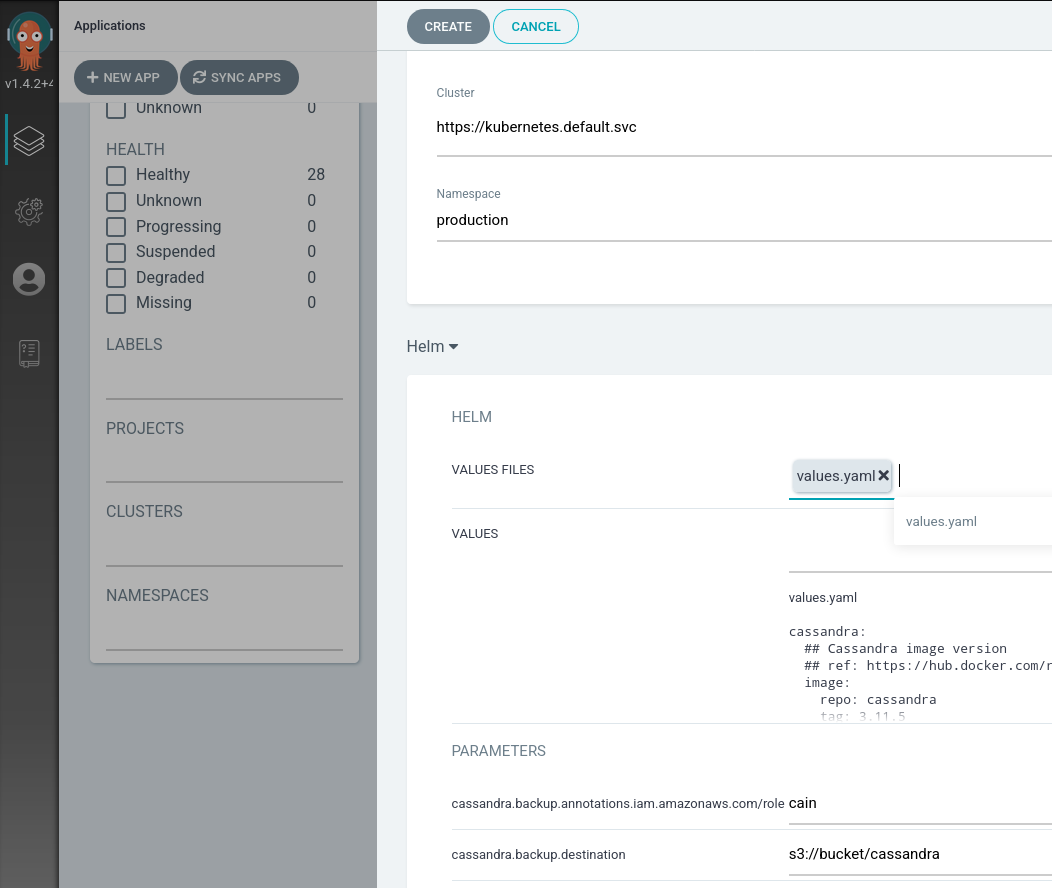
\includegraphics[width=1.0\textwidth]{images/primer-uporabe-helm-predloge-argo-cd.png}
\end{center}
\caption{Primer uporabe helm predloge v ArgoCD.}
\label{primer-uporabe-helm-predloge-argo-cd}
\end{figure}


\section{KubeFed}
9. 1. 2018 je bil po propadlem projektu Kubernetes Federation V1 ustvarjen Kubernetes Federation V2 ali KubeFed~\cite{Kubernetes-federation-evolution}.
Oba projekta sta želela poenostaviti upravljanje večih klastrov in razporejanje Kubernetes objektov.
V projektu Federation V1 je bil ubran pristop, ki je skupino klastrov ali federacijo uporabniku predstavil kar kot nov klaster~\cite{setup-cluster-federation-kubefed-v1}.
Uporabljal je svoj API in api kontroler, ki pa je bil združljiv s Kubernetesovim, kar pa je omogočalo tudi uporabo orodja kubectl~\cite{cluster-federation-in-Kubernetes-1.5}.
Objekti, ki jih je federacija podpirala so bili kompatibilni s standardnimi Kubernetes objekti~\cite{federated-cluster-kubefed-v1}.
Takšne objekte je potem Federation V1 ustvaril tudi v ostalih klastrih.
Zanimiv pristop, ki pa zaradi mnogih pomankljivosti in pomankanja možnosti naprednejših konfiguracij ni uspel pridobiti statusa GA.

Tako se je kasneje rodil projekt Federation V2~\cite{Kubernetes-federation-evolution}.
Glavna razlika s prvo verzijo z uporabniškega stališča je v tem, da za federacijo ne poizkuša imitirati Kubernetesovega API, ampak uporablja obstoječi Kubernetesov API. 
Federation V2 samo predstavi nove objekte, ki pa so razširitev standardnih, kot naprimer federateddeployment.
Federated objekte je treba najprej vklopiti s komando kubefedctl enable.
\begin{verbatim}
kubefedctl enable deployment
\end{verbatim}
Orodje kubefedctl si moramo namestiti na naš računalnik.
Takšen Federated objekt vsebuje tri glavne lastnosti: definicija predloge primarnega objekta, postavitev v klastre in prepis lastnosti originalnega objekta za posamezne klastre.
  Takšen pristop je zelo široko zastavljen in omogoča tudi federacijo CRD objektov.
\begin{verbatim}
apiVersion: types.kubefed.io/v1beta1
kind: FederatedDeployment
spec:
  placement:
    clusterSelector:
      # izbira klastrov
      matchLabels: {}
      ... 
  template:
    # specifikacije deployment objekta
    spec:
    ... 
  overrides:
    # prepis konfiguracije za posamezne klastre
    - clusterName: klaster1
      clusterOverrides:
          # nastavi polje replicas na vrednost 5
        - path: "/spec/replicas"
          value: 3
  ... 
\end{verbatim}
  Federation V2 podpira poleg sinhronizacije infrastrukture tudi odkiravnje storitev v drugih klastrih prek DNS zapisov.
Ampak se omenja možnost odstranitve te funkcionalnosti~\cite{remove-service-discovery}, ki je že sedaj privzeto izklopljena.
  Preden pa uporabimo KubeFed pa se moramo zavedati, da je projekt v času pisanja diplomske naloge še vedno v razvojni fazi alfa in lahko mine še nekaj časa preden bo na voljo splošni javnosti(GA), če slučano ne bo šel po stopinjah svojega predhodnika.
\section{Cilium}
Cilium je odprtokodni program, ki nam omogoča napredne varnostne in omrežne nastavitve v našem klastru~\cite{cilium-intro}.
Program deluje na tretji in četrti omrežni plasti, kjer nam zagotavlja osnovne principe varnosti in zaščite.
Tu govorimo o zapiranju portov in omejevanju prometa.
Cilium pa nam zagotavlja tudi naprednejšo varnost na sedmi omrežni plasti, saj nam omogoča naprimer omejevanje in filtriranje HTTP zahtevkov in podobne varnostne funkcije na popularnih protokolih aplikacijskega nivoja~\cite{cilium-intro}.

Ker Cilium implementira precejšni del mreženja in povezovanja v Kubernetesu, pa nam s tem lahko ponudi tudi nekaj zelo naprednih možnosti, ko med seboj povezujem več različnih klastrov Kubernetes.
Tako nam kot ključno prednost Cilium omogoča tudi komunikacijo med podi v različnih klastrih~\cite{cilium-cluster-mesh} in uporabo globalnih objektov service, ki so sposobni delati razporejanje prometa med različnimi klastri.
Takšne objekte definiramo z anotacijo io.cilium/global-service~\cite{setup-cilium-cluster-mesh}.
Omogoča nam tudi omejevanje povezovanja med klastri z njihovim objektom CiliumNetworkPolicy~\cite{setup-cilium-cluster-mesh}.
Ko postavljamo mrežo klastrov, pa se moramo še vedno zavedati, da Cilium ne rešuje problema, če so naši klastri skriti v različnih privatnih omrežjih.
Ključno pri uporabi Ciliuma za povezovanje klastrov je, da so vsa naša vozlišča dosegljiva med seboj.
A četudi so naši klastri v med seboj nedosegljivih privatnih omrežjih, pa je problem z lahkoto rešljiv z uporabo sistema VPN, ki nam omogoča, da vsa vozlišča povežemo v eno virtualno omrežje~\cite{setup-cilium-cluster-mesh}.

Kljub naprednim funkcijam, ki nam jih Cilium ponuja, pa se moramo zavedati, da se Cilim ukvarja samo s povezovanjem klastrov na omrežnem nivoju.
Ne omogoča enotnega upravljanja in sinhroniziranja objektov med klastri zato moramo objekte sinhronizirati sami.
Ampak zaradi dovolj široke zasnove Kubernetesovega vmesnika so rešitve med seboj kompatibilne.
Torej lahko uporabimo napredno mreženje Ciliuma in sinhronizaciramo objekte s KubeFed in GitOps pristopom.
\chapter{Priprava sistema klastrov za testiranje}
\section{Raspberry PI 4}
Za namene testiranja različnih načinov povezovanja klastrov Kubernetes moramo najprej postaviti nekaj klastrov Kubernetes.
Zaradi preprostosti in nizke cene, predvsem pa ker se koncepti zaradi tega ne spremenijo bomo za naša Kubernetes vozlišča uporabili Raspberry PI 4.
  Na višjem nivoju je neglede na vse naš klaster in je delo zelo podobno, če uporabimo nekaj 1000 vozlišč v klastru v oblaku ali pa lokalni klaster z enim vozliščem.
Raspberry PI je zelo majhen in manj zmogljiv računalnik na eni sami plošči.
Ključni prednosti takšnih računalnikov pa sta prav velikost in cena.
Na vsak Raspberry PI se bo namestil Kubernetes klaster z enim samim vozliščem.
Fizična postavitev klastrov je prikazana na sliki \ref{rpi-klastri}.
\begin{figure}[h]
\begin{center}
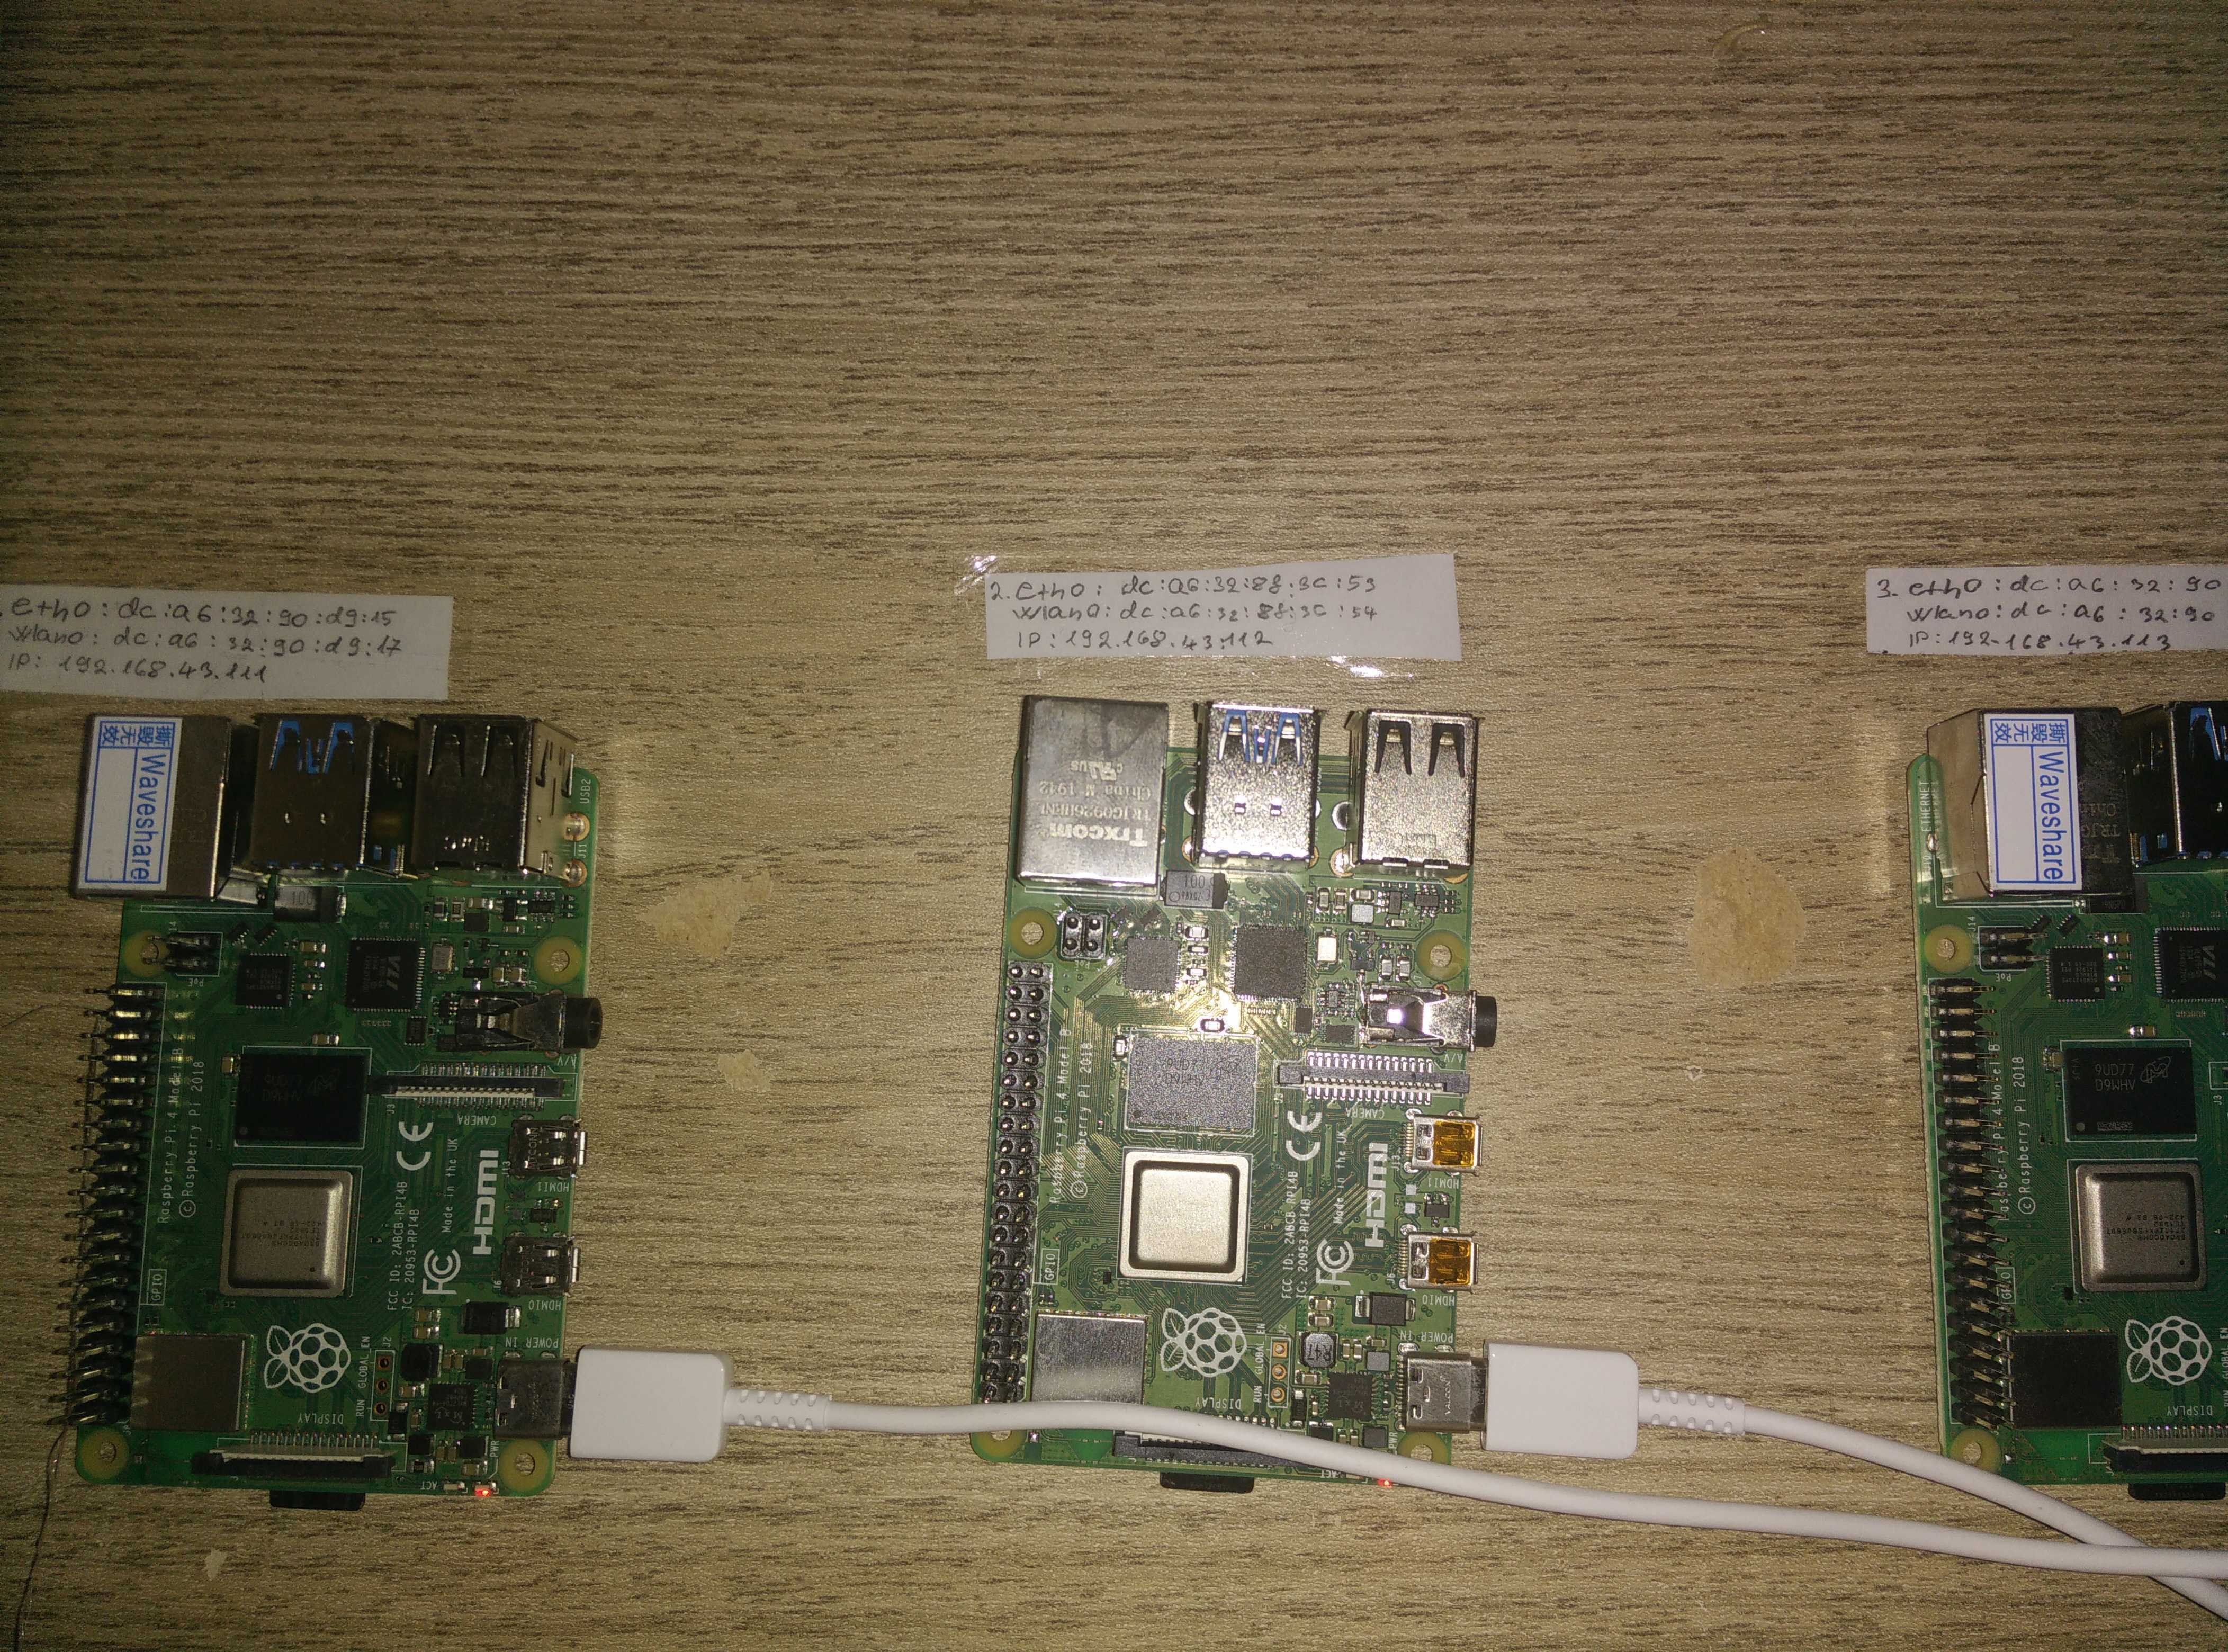
\includegraphics[width=1.0\textwidth]{images/postavitev-raspberry.jpg}
\end{center}
\caption{Postavitev raspberry klastrov.}
\label{rpi-klastri}
\end{figure}
\section{K3S in K3OS}
Obstaja več implementacij Kubernetesa in mi bomo uporabili z viri varčno odprotokodno implementacijo K3S od podjetja Rancher~\cite{k3s-info}.
Hkrati so v podjetju Rancher pripravili distribucijo operacijskega sistema Linux K3OS, ki jo lahko namestimo na katerikoli računalnik~\cite{k3os-git}. 
Majhna težava se pojavi, ker še ni pripravljene uradne verzije operacijskega sistema za ploščice Raspberry PI.
A k sreči se je v ta namen začel odprtokodni projekt PiCl k3os image generator, ki nam iz slik operacijskih sistemov K3OS in Raspberry OS in konfiguracijskih datorek zgradi novo sliko operaijskega sistema za naš Raspberry PI ~\cite{k3os-rpi-image-generator}.
Konfiguracijske datoteke, ki jih moramo priložiti so standardne YAML datoteke, ki jih podpira K3OS.
Vanje zapišemo nastavitve kot so ssh javni ključi za dostop, podatki od WiFi omrežja na katerega se povezujemo, geslo, žeton za povezavo z Kubernetes klastrom in način v katerem želimo zagnati K3S na sistemu~\cite{k3os-git}.
\begin{verbatim}
ssh_authorized_keys:
- ssh-rsa ...
hostname: klaster-1
k3os:
  ntp_servers:
  - ...
  password: ...
  token: ...
  dns_nameservers:
  - ... 
  wifi:
  - name: ...
    passphrase: ...
  k3s_args:
  - server
\end{verbatim}
V našem primeru smo vse K3S programe zagnali v strežniškem načinu in nobenega v načinu delovnega vozlišča, saj želimo, da vsak Raspberry PI predstavlja svoj klaster.
\section{Demonstracijska spletna aplikacija}
Za potrebe testiranja je bilo potrebno naredili novo testno mikrostoritev.
Ker se v tem diplomskem delu želimo osredotočiti na resnične probleme v industriji, mora ta aplikacija omogočati tudi shranjevanje podatkov v podatkovno bazo.

Koda, ki je javno objvaljena v Git repozitoriju~\cite{git-stateful-rest-sample}, je napisana v programskem jeziku Go.
Iz kode je bil zgeneriran kontejner, ki je objavljen v javnem Docker repozitoriju~\cite{docker-stateful-rest-sample}.
Ob tem velja opozoriti, da Raspberry PI uporablja ARM arhitekturo procesorja, kar je zahtevalo posebno pozornost.

Aplikacija deluje preprosto.
Na mrežnih vratih podanih z okoljsko spremenljivko izpostavi vmesnik REST z dvema preprostima HTTP klicema.
GET klic na pot /users nam bo vrnil vse uporabnike, ki so zapisani v tabeli v bazi, s klicem POST na isto pot pa poskrbimo, da se podatki uporabnika iz našega zahtevka shranijo v tabelo v bazo.
\begin{verbatim}
# ukaz za dodajanje uporabnika
curl -X POST localhost/users --data '{"name": "John", "lastname": "Doe"}'
# ukaz za prikaz vseh uporabnikov
curl localhost/users
\end{verbatim}

Za shranjevanje podatkov bomo uporabili 2 različni SQL bazi podatkov.
Postgres, ki je preprosta za lokalni razvoj, a ne omogoča napredne sinhronizacije podatkov med strežniki in CrateDB, ki je bil zasnovan kot SQL baza na več vozliščih in nam omoča napredne sinhronizacije tudi med različnimi strežniki in klastri.
K sreči pa CrateDB implementira PostgreSQL vmesnik in nam kode za prehod med bazami ni potrebon spreminjati.
\section{Namestitev KubeFed}
Kot ena izmed ključnih komponent složnega delovanja večih klastrov je njihovo upravljanje.
V te namene bomo uporabili program KubeFed, ki ga moramo namestiti na enega izmed klastrov, ki jih želimo povezati skupaj.
Ker je izdelek še v razvoju in še ni prišel iz alfa faze nimajo objavljene verzije za procesorje ARM.
Zato je bilo iz kode KubeFed potrebno zgraditi novo sliko kontejnerja, ki je javno objavljena~\cite{docker-kubefed}.
Potem pa smo uporabili originalno Helm predlogo, kjer smo samo zamenjali originalno sliko kontejnerja z našo.
Za delo s KubeKed pa moramo na svoj računalnik namestiti orodje kubefedcli.
Z uporabo ukaza kubefedctl join povežemo vse tri klastre v kubefed sistem.
\begin{verbatim}
kubefedctl join klaster-1
kubefedctl join klaster-2
kubefedctl join klaster-3
\end{verbatim}
S tem smo uspešmo povezali več klastrov Kubernetes v sistem KubeFed.
\chapter{Povezovanje med podatkovnimi centri}
\section{Problem velike latence}
V industriji je zelo malo primerov spletna aplikacije, ki jim ni potrebno hraniti stanja. 
Ko neko podjetje, lastnik aplikacije poseže po globalnem trgu zelo hitro ugotovi, da stranke, ki niso blizu podatkovnega centra precej dlje čakajo pred ekrani, da se naloži njihova spletna aplikacija in njihovi podatki.
Takšen problem se v splošnem rešuje tako, da našo aplikacijo postavimo še na dodaten strežnik bližje uporabniku. 
Rešitev se sliši preprosta, a vseeno se tu srečamo z zelo zahtevnimi problemi v računalništvo.
Najbolj očiten primer je sinhronizacija podatkov.
V našem primeru bomo uporabili podatkovno bazo CrateDB~\cite{cratedb}, novejšjo alternativo standardnim SQL podatkovnim bazam.
CrateDB ima v primerjavi s tradicionalnimi podatkovnimi bazami, boljšo podporo za sinhornizacijo podatkov med vozlišči.
Poleg vsega pa nam za uporabo podatkovne baze CrateDB ni potrebno konceptualno spreminjati naše aplikacije, saj podpira vmesnik od base PostgreSQL.
\section{Povečanje dosegljivosti aplikacije}
Če je čim višja dosegljivost za našo aplikacijo kritičnega pomena in smo že poskrbeli za visoko dosegljivost (HA) aplikacije v našem klastru, še vedo lahko pride do situacije, ko iz omrežja izpade cel podatkovni center.
Spomnimo, da je ena izmed zahtev, za učinkovito delovanje Kubernetesa, postavitev strežnikov blizu skupaj.
V primeru naravnih nesreč ali hujših vremenskih pogojev pomeni, da je nedosegljiv cel podatkovi center in s tem klaster v njem.
Če uporabljamo oblak, pa gremo lahko še korak dlje z zagotavljanjem dosegljivosti.
Če nam ni dovolj niti, da uporabimo različne dosegljivostne cone in podatkovne centre oblačnih ponudnikov, lahko postavimo naše klastre pri več različnih ponudnikih.
Tu Kubernetes pride zelo do izraza, saj kljub nekaj neenakostim skozi implementacije ohranja enak vmesnik in je zato takšna postavitev precej lažja, kot bi bila brez uporabe Kubernetesa.
\section{Povezovanje klastrov Kubernetes med podatkovnimi centri}
Rešitev za oba problema je identična.
Postaviti moramo klastre v več različnih podatkovnih centrov in jih nastaviti, da bodo delovali sinhrono.
Odvisno od problema bodo te podatkovni centri morda bližje uporabniku, morda v lasti različnih oblačnih ponudnikov ali pa oboje.
Ampak princip ostaja enak.
\section{Razporeditev uporabnikov po klastrih}
Ko imamo na vsakem klastrih javno izpostavljen service in urejene ingress zapise moramo še vedno uporabnike preusmeriti na njim najbljižji klaster.
Uporabnike lahko mi usmerimo avtomatsko z DNS zapisi, ki omogočajo usmerjanje na podlai geolokacije.
Lahko uporabimo in namestimo zunanju DNS skozi Kubernetes ali pa kar ročno.
\begin{figure}[h]
\begin{center}
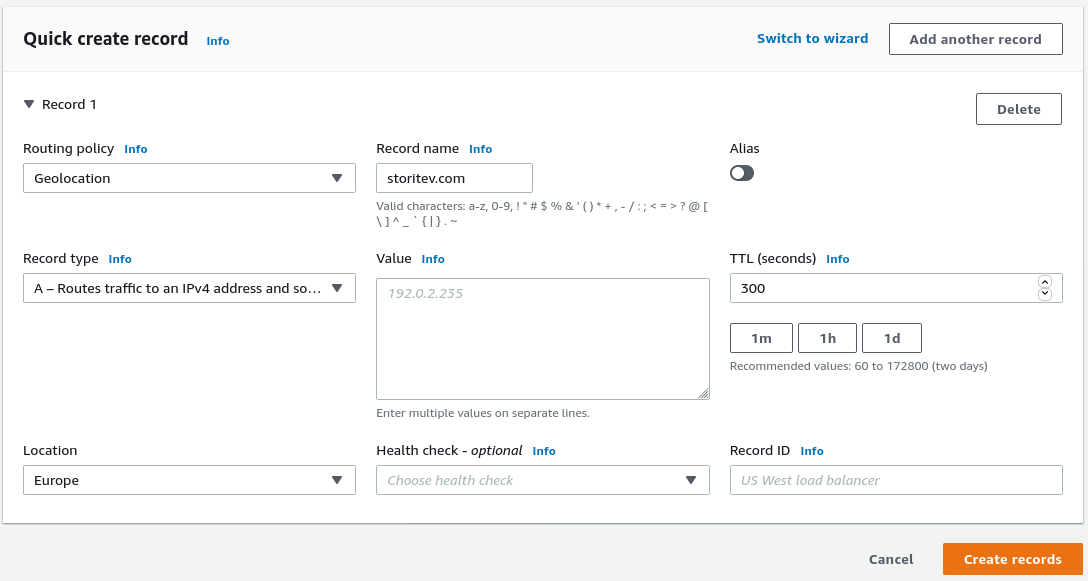
\includegraphics[width=1.0\textwidth]{images/geolokacijski-dns.png}
\end{center}
\caption{Ustvarjanje geolokacijskega DNS zapisa v storitvi ROUTE53.}
\label{primer-ustvarjanje-geolokacijskega-zapisa}
\end{figure}
V naših lokalnih testnih klastrih bomo ta korak preskočili in jih ne bomo usmerjali preko javnih dns strežnikov, saj v lokalnem okolju to ni smiselno.

Naslednja možnost pa je rešitev, ki se jo zelo pogosto poslužujejo internetne računalniške igre, da so naši strežniki popolnoma ločeni in se vsak uporabnik sam odloči na katerem klastru ali strežniku želi igrati.
V takšnih primerih se ponavadi tudi izognemmo problemu sinhronizacije podatkov med strežniki, kar zelo poenostavi upravljanje naših klastrov.
\section{Infrastruktura primera}
V našem primeru spletne aplikacije bomo imeli v vsakem klastru en deployment z našo aplikacijo Stateful rest sample in en pripadajoči service, da aplikacijo izpostavimo izven klastra.
Za podatkovno bazo pa bomo uporabili statefulset s CrateDB, diskom na lokalni SD kartici, internim servicom za prepoznavo ostalih instanc CrateDB v klastru in eksterni service, ki ga uporabimo za povezovanje na podatkovno bazo.
\begin{figure}[h]
\begin{center}
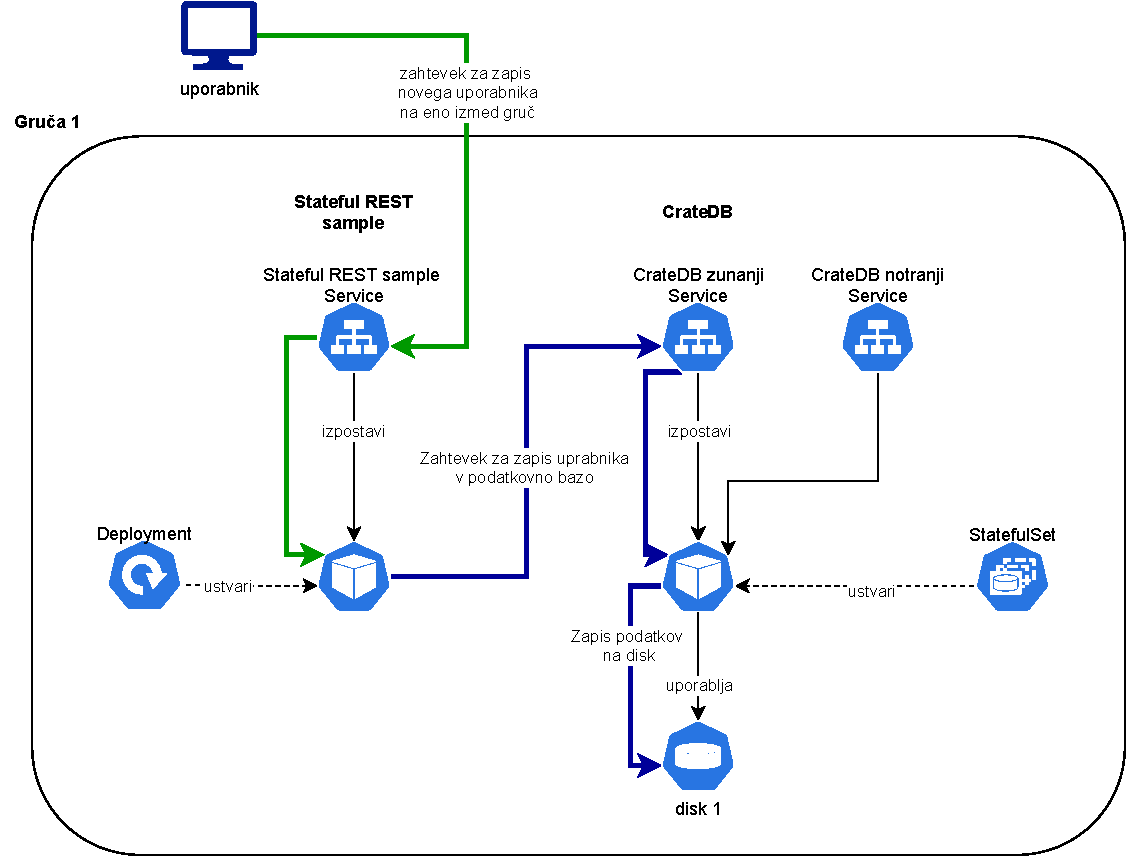
\includegraphics[width=1.0\textwidth]{images/infrastructure-example.pdf}
\end{center}
\caption{Infrastruktura vsakega klastra v primeru demonstracijske aplikacije}
\label{primer-uporabe-helm-predloge-argo-cd}
\end{figure}
Vsa konfiguracija je javno objavljena na Git repozitoriju\cite{git-diploma}. Postavimo jo z ukazom.
\begin{verbatim}
kubectl apply -f diploma-demo-1
\end{verbatim}
Takoj preverimo, ce aplikacija deluje in če lahko podatke zapisujemo v bazo, tako da prek demo aplikacije poizkusimo dodati uporabnika in izpisati vse uporabnike. To naredimo z curl komando.
\begin{verbatim}
curl -X POST klaster-1/users --data '{"name": "John", "lastname": "Doe"}'
curl klaster-1/users
\end{verbatim}
\section{Implementacija infrastrukture s KubeFed}
Najprej se moramo odločiti za katere tipe objektov bomo vklopili federacijo oziroma za katere bomo želeli univerzalno upravljanje.
V našem primeru gre za service, deployment in statefulset. Vklopimo jih z naslenjim ukazom, ki za nas ustvari nove federated tipe objektov na izbranih tipih.
\begin{verbatim}
kubefedctl enable <ime tipa>
\end{verbatim}
Ko smo si vklopili federacijo na vseh potrebnih tipih pa moramo še vklopiti avtomatsko upravljanje na specifičnih objektih.
V našem primeru želimo za to uporabiti ukaz kubefedctl federate.
\begin{verbatim}
kubefedctl federate deployment stateful-rest-sample
kubefedctl federate service stateful-rest-sample
kubefedctl federate statefulset crate
kubefedctl federate service crate-internal
kubefedctl federate service crate-external
\end{verbatim}
Izvršeni ukazi ustvarijo federated objekte, ki uporabijo postavitev vse klastre in za predlogo kar podane objekte.
Tako je za nas rezultat izvršenih ukazov kreiranje federated objektov in posledično kopiranje objektov v vse naše povezane klastre.

Po preizkusu delovanje s curl komando opazimo, da podatki med klastri še vedno niso sinhornizirani.
Uporabniki, ki jih vnesemo v en klaster se še ne sinhronizirajo v ozadnju.
Na tej točki se ustavijo nekatere spletne aplikacije in prepustijo izbiro strežnika oziroma klastra kar uporabniku.
\section{Sinhronizacija podatkov}
Če želimo pred uporabnikom skriti, da uporabljamo več klastrov, moramo poleg geolokacijskih DNS zapisov, urediti tudi avtomatsko sinhronizacijo podatkov.
Sicer v našem primeru res uporabljamo samo eno instanco CrateDB baze na klaster a vseeno smo na nivoju sinhronizacije znotraj klastra to stvar že uredili. 
Zopet se moramo spomniti, da so tudi klastri podatkovnih baz ponavadi narejeni tako, da najbolje delujejo, če so vozlišča blizu skupaj.
Zaradi tega mnoge baze, ki podpirajo sinhronizacijo podatkov znotraj klastra, podpirajo tudi sinhronizacijo med različnimi podatkovnimi centri.
\subsection{Uporaba primerne podatkovne baze}
Najlažje je sinhronizirati podatke, če uporabimo podatkovno bazo, ki ima sinhronizacijo med različnimi klastri s čim manj dela že podprto.
CrateDB podpira sinhronizacijo tudi preko dosegljivostnih con.
Vseeno pa je mišljeno, da vsa vozlišla povežemo v enak podatkovni klaster.
To pomeni, da morajo vsa vozlišča imeti dostop do vseh.
Zelo elegantna rešitev bi bila uporaba sistema Cilio in uporaba globalnih servicov, saj nam Cilio že omogoča komunikacijo vsakega poda z vsakim.
Druga možnost pa je, da izpostavimo vsak pod s svojim javnim IPjem in jih ročno povežemo v klaster.

Potem pa moramo nastaviti še nastavitve, ki ki jih baza podpira za zmanjšanje prometa in zagotavljanje željenje dosegljivosti med klastri~\cite{cratedb-zone}.
Podobne načine sinhorinzaije podpira tudi naprimer podatkovna baza Cassandra~\cite{cassandra-zone}.
\subsection{Podatke sinhroniziramo sami}
Sinhronizacija podatkovne baze je tažak problem.
Če ne uporabimo primerne podatkone baze ali pa želimo sinhronizirati samo določene stvari preko klastrov bomo sinhronizacijo podatkov verjetno morali napisati sami.
To pomeni, da bomo ustvarili novo mikrostoritev, ki bi v ozadju kopirala ključne podatke med podatkovnimi centri.
Ker samo mi poznamo naš konkreten primer uprabe, je takšen pristop pogosto najbolj učinkovit s stališča prenosa podatkov.

V našem primeru bomo s preprosto skripto kopirali uporabnike iz ene aplikacije v drugo, kar z uporabo našega REST apija.
To bomo storili v drugem ubuntu kontejnerju z uproabo komand curl za izvajanje rest api klicev in jq za razčlenjevanje podatkov.
Podatki se sinhronizirajo vsakih 10 sekund.
Ker naša aplikacija ne omogoča brisanja podatkov je takšen pristop učinkovit.

Primer še testiramo in dobimo spodnji izhod, kar potrdi, da so se podatki uspešno sinhronizirali.
\begin{verbatim}
curl -s -X POST klaster-1/users|jq --data '{"name": "John", "lastname": "Doe"}'
curl -s klaster-2/users|jq
[{"Name":"John","Lastname":"Doe"}]
\end{verbatim}
\chapter{Upravljanje izoliranih aplikacij}
\section{Zmanjševanje posledic vdorov in izpadov}
Računalniška stroka si je že nekaj časa nazaj priznala, da popolnega sistema ne more ustvariti.
Sistema, ki se ne more sesuti, sistema, ki bo ves čas dosegljiv in sistema v katerega ne bo mogoče vdreti.
To vsake toliko časa potrdijo največji igralci z izpadi ali vdori na njihovih storitvah. 
Vsake nekaj časa pa se vseeno pojavi podjetje, ki trdi da vdor k njim ni mogoč in so vsakič znova prepričani v nasprotno.
Vseeno pa kljub temu, da so vdori in napake, zaradi katerih postanejo nedosegljivi naši klastri vedno lahko poizkusimo zmanjšati posledice ob morebitnem vdoru ali napadu. 
\subsection{Izpadi aplikacije}
Kljub temu, da smo naše aplikacije namestili na različne klastre in je s tem aplikacija odporna na izpad enega klastra pa ob hujših nepravilnostih delovanja aplikaije in nastavitev klastra lahko zaradi napake na eni aplikaciji izpadejo vsi klastri na katerih imamo aplikacijo nameščeno.
Takšen primer bi bil, če ena aplikacija ali mikrostoritev zavzame vse vire na klastru hkrati pa odpovejo ostale varovalke, ki jih ponuja že sam Kubernetes.
V takšnih primerih bo odpovedal cel naš sistem namesto samo del sistema.
Zato se lahko odločimo, da bomo nekatere bolj kritične aplikacije ali mikrostoritve postavili v klaster, kjer napake drugih aplikacij ne bodo vplivale na naše delovanje.
A vseeno se moramo zaveati, da je ta korak smiselen šele ko smo opravili že vse predhodne preventivne ukrepe, kot so razdelitev aplikacije na mikrostoritve, kontejnerjizacija, izolacija na posamezno Kubernetes vozlišče, pravilna nastavitev omejitev avtomatskega povečevanja in še mnoge druge.
\subsection{Vdori}
Podobno kot pri izpadih aplikacije pa je pri preprečevanjih posledic vdorov.
Najprej moramo poskrbeti za primerno zaščito Kubernetes vozlišč, naše aplikacije, enkripcija komunikacije med mikrostoritvami, uporaba nepriviligiranih kontejnerjev.
Če pa nam vsi zgoraj našteti in ostali priporočeni ukrepi niso dovolj ali pa se zavedamo, da imamo v klastru manj varne aplikacije in napadalec prek teh aplikacij ne sme dostopati do podatkov kritičnih aplikacij, potem je smiselno kritične aplikacije izolirati v svoj klaster.
\section{Implementacija s Kubefed}
Ključna lastnost federiranih objektov je možnost izbire klastov na katerih se bo določen objekt ustvaril. 
S tega stališča je naš primer zelo preprost.
Samo določimo da se naša aplikacija izvaja na klastru 3 namesto na vseh.
Tokrat za federacijo ne moremo uporabiti ukaza kubefedctl federate, ampak moramo kot za vse ostale Kubernetes objekte spisati konfiuracijo.
Najprej bomo z ukazom kubectl tag označili naš izoliran klaster (ali več njih).
Potem pa bomo lastnosti vsakega spec.placement.clusterSelector.matchLabels federiranega objekta, ki ga želimo izolirati dodali označbo vseh izoliranih klastrov.
V takšnih primerih se nam ni potrebno posebej ukvarjati s sinhronizacijo podatkov, saj ali smo vse podatke obdržali v istem klastru ali pa sinhroniziramo na enak način kot če sinhroniziramo med različnimi podatkovnimi centri.
\chapter{Upravljanje klastrov na robu oblaka}
\section{Klaster na robu oblaka}
Razlogov zakaj klastre postavljamo na rob oblaka oziroma fizično bližje končnemu uporabniku je več.
Pogosto želimo na glavni strežnik pošiljati vseh podatkov ampak jih obdelovati že lokalno, da ne prenašamo po omrežju vseh podatkov.
Smiselnost takšne postavitve pride še posebej do izraza, če podatke prenašamo bo dragem mobilnem omrežju
A možnih postavitev in razlogov zanje je res veliko.
Naprimer lahko gre za zahteve strank, da se podatki obdelujejo lokalno, lahko gre za zakonske omejitve lahko želimo operacije izvajati na napravah, ki si jih ne lastimo direktno itd.

V našem primeru se bomo osredotočali na upravljanje takšnih klastrov.

\section{Implementacija s KubeFed}
Ko enkrat povežemo vse klastre s kubefedctl join je njihovo upravljanje preprosto.
Samo nastavimo v katerem klastru želimo katere objekte in naša naloga je končana.
Zavedati se sicer moramo, da nekaj komunikacije porabi tudi KubeFed za sinhronizacijo.

Nam pa KubeFed omogoča še eno lepo možnost s svojo strukturo, saj je vsak od federiranih objektov v svojem imenskem prostoru.
Tako lahko s svojim kontrollerjem in KubeFed apijem implementiramo še dodatne funkcijonalnosti kot so razporejanje obramenjenosti med lokalnimi strežniki in po potrebi povečujemo število instanc ali pa kar razporejamo opravila s Kubernetes Jobi.

Z zelo preprosto integracijo v Kubernetes nam KubeFed api tu res omogoča zelo preprosto implementacijo katerekoli naše rešitve.
\section{Sinhronizacija podatkov}
asdf V primeru klastrov na robu oblaka se sinhronizacijo praviloma vedno implementira na novo, saj le mi vemo kakšen problem rešujemo in zakaj smo sploh postavljali klastre na robu oblaka.


\chapter{Sklepne ugotovitve}
Uporaba \LaTeX{a} in \BibTeX{a} je v okviru Diplomskega seminarja \textbf{obvezna}!
Izbira \LaTeX\ ali ne \LaTeX\ pri pisanju dejanske diplomske naloge pa je pre\-pu\-šče\-na dogovoru med vami in vašim mentorjem.
Res je, da so prvi koraki v \LaTeX{}u težavni. 
Ta dokument naj vam služi kot začetna opora pri hoji.
Pri kakršnihkoli nadaljnih vprašanjih ali napakah pa svetujem uporabo Googla, saj je spletnih strani za pomoč pri odpravljanju težav pri uporabi \LaTeX{}a ogromno.
\newpage %dodaj po potrebi, da bo številka strani za Literaturo v Kazalu pravilna!
\ \\
\clearpage
\addcontentsline{toc}{chapter}{Literatura}
\bibliographystyle{plain}
\bibliography{literatura}
\end{document}
